\section{Evaluation}
\label{sec:evaluation}
DFiant aims to greatly improve designer productivity. To evaluate possible productivity gains we chose several open-source RTL projects and implemented them in DFiant: an AES cypher, an IEEE-754 double precision floating point multiplier, a RISC-V single-cycle core, a bitonic-sort network, and other simple examples.
We compared the DFiant implementations with their RTL counterparts as follows:
\begin{enumerate}[leftmargin=*]
	\item \textit{Conciseness}\quad The DFiant code is significantly more compact than the RTL code (from 50\% to 70\% less code), because DFiant semantically implies much of the additional information required by the RTL description. Most prominently, the RTL code differentiates between registers and wires, requires explicit pipeline register placement, and adds stall control logic. 
	\item \textit{Portability, Performance, and Correctness}\quad An RTL implementation for a given functionality is but one of many possible RTL representations that vary when different device and performance constraints are required and therefore can be considered \textit{correct} only when those conditions are true, whereas the DFiant design remains unchanged and can be considered always correct once verified. 
	\item \textit{Debugging and Legibility}\quad A DFiant design generated RTL code maintains a readable, true to the source, format, by maintaining the intended names and structure expressed in the original DFiant design, unlike cryptic codes generated by many HLS and high-level design tools. However it is still harder to debug RTL code generated by DFiant than an RTL code written by a human designer.
\end{enumerate} 

%{Brainstorming}
%Explicitly saving history for sample
%Thanks to type inference, no need to declare types for internal values.
%No need to extend the a value to get a carried result.
%No need to create explicit pipeline (which also changed according to the target device).
%No need to explicitly create stall logic.
%We are replacing concepts of register and wire to state and stateless. This is key difference between dataflow 
%and RTL HDLs. Dataflow assumes there is always a history, in every dataflow value. So we can access the history, yet call it stateless.



%\subsection{Methodology}
%
%
%We chose the following comparison metrics: the maximum clock frequency, clock cycle latency, utilizations of both look-up tables (LUTs) and flip-flop registers (FFs), and lines of code (LoC). Digital signal processing (DSP) block utilization was zero for AES and equivalent for FPMul across all designs, thus neglected from the table. We used Xilinx Vivado to synthesize and implement the RTL design for a Virtex-7 FPGA, part number: xc7vx485tffg1761-2. The tool was configured to use default strategy for both synthesis and implementation processes. For each design, we recorded the maximum clock frequency, LUTs, and FFs. We recorded the design latency as reported by the DFiant and Vivado HLS compilers, and the RTL cores documentation. Finally, we automatically counted the LoC \cite{danial2009cloc}, applied standard score normalization (0-100) to all metrics, and assured higher values indicate better score for all metrics. Mean score of all metrics is presented as well.
%
%\subsection{Case Study: AES Cypher}
%For baseline comparison we used three AES cypher RTL designs from opencores.org: Das core \cite{das2010fully}, Hsing core \cite{hsing2013aes} and Salah core \cite{salah2013aespipe}. Additionally, we obtained a Vivado C++ HLS design~\cite{oflynn2014rapid}. All these designs are fully pipelined, meaning that in every cycle the design accepts new key and data inputs, and emits an encrypted data output, delayed by a fixed design latency.
%
%We compiled the DFiant and Vivado HLS designs with three target clock frequencies: 200 MHz, 300 MHz, and 450 MHz. We named the designs accordingly (e.g., DFiant\_200 is the 200MHz target design). We collected the results in Table~\ref{tbl:AES_Compare_Table}, and displayed their normalized standard score in Fig.~\ref{fig:AES_Compare_Graph}. We added the supported key types quantity as a metric, since some designs support 128bit keys and do not include 192bit and 256bit keys as well. The table also includes an 'SBox BRAM Use' column, since some designs do not use memory to implement the AES SBox function.
%
%%\begin{table*}[t!]
%%  \centering
%%  \begin{minipage}[t][5cm][t]{0.62\linewidth}
%%    \centering
%%    \captionof{table}{AES Cypher RTL Designs Comparison\\(the numbering on the left associates configurations with \fig{fig:AES_Compare_Graph})}
%%    \label{tbl:AES_Compare_Table}
%%    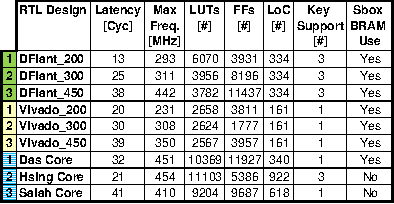
\includegraphics[scale=1]{graphics/AES_Compare_Table.pdf} 
%%  \end{minipage}
%%  \hfill
%%  \begin{minipage}[t][5cm][t]{0.37\linewidth}
%%    \centering
%%    \captionof{table}{FP Mult. RTL Designs Comparison\\(the numbering on the left associates configurations with \fig{fig:FP_Compare_Graph})}
%%    \label{tbl:FP_Compare_Table}
%%    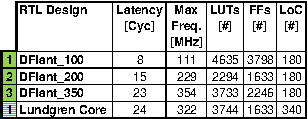
\includegraphics[scale=1]{graphics/FP_Compare_Table.pdf} 
%%  \end{minipage}
%%  \begin{minipage}[b][3.8cm][b]{0.62\linewidth}
%%  	\centering
%%    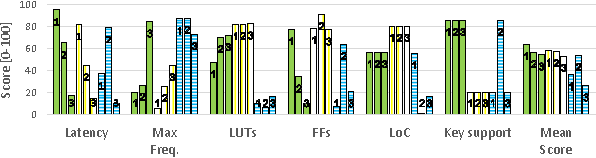
\includegraphics[height=3cm]{graphics/AES_Compare.pdf} 
%%    \captionof{figure}{AES cypher RTL designs score comparison (higher = better)\\ \quad}
%%    \label{fig:AES_Compare_Graph}
%%  \end{minipage}
%%  \hfill
%%  \begin{minipage}[b][3.8cm][b]{0.37\linewidth}
%%    \centering
%%    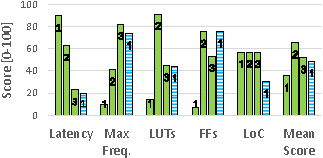
\includegraphics[height=3cm]{graphics/FP_Compare.pdf} 
%%    \captionof{figure}{FP multiplication RTL designs score comparison (higher = better)}
%%    \label{fig:FP_Compare_Graph}
%%  \end{minipage}
%%\end{table*}
%
%The Hsing core clearly has the best performance among the different designs (but the lowest score on LUTs utilization). The primary reason it achieved this is because it uses LUTs instead of BRAMs. This enables the synthesizer to optimize the AES SBox function, and even pipeline it. DFiant uses its \code{lookupTable} library function to implement SBox, and we have yet to enable such an option for DFiant. 
%
%Although the DFiant-generated RTL performance is not optimal, it can still  be improved without modifying the DFiant AES code, if the DFiant compiler is optimized. Moreover, this code has an adaptive pipeline, while the RTL cores pipelines are fixed. The Vivado implementation enjoys the same advantages as DFiant, and has even less LoC. However, the Vivado code does not support all possible keys and its maximum performance is far from optimum (we did not attempt to improve the HLS pragma directives).
%
%If we assume all metrics have the same weight, the mean score places the DFiant solutions at the top. It is difficult to determine what is truly the best solution, but DFiant clearly has the best potential for further improvement without any modification to the application code.
%
%           
%\subsection{Case Study: Double Precision FPMul}
%
%We compared our FPMul with the open IEEE-754 compatible Lundgren core \cite{lundgren2014open} (the only IEEE-754 fully compatible FPMul RTL design we had access to). Since the core is a complete floating point unit, we disabled the unnecessary parts, reducing it to only an FPMul, for a fair comparison with DFiant's code. The DFiant code was written by using the Lundgren VHDL code as a reference design. The designs are very similar in their structure, except that DFiant is considerably less verbose, and has no explicit pipeline.
%
%We had no access to an open Vivado HLS FPMul for comparison. We could have directly invoked a \code{double} multiplication, but an inspection of the generated RTL revealed that Vivado HLS just instantiates an RTL floating point blackbox core. DFiant can choose to use this core as well, and achieve identical performance to Vivado HLS. Furthermore, the Vivado HLS floating point implementation is not fully compatible with IEEE-754 (e.g, does not support denormalized numbers).
%
%Similarly to the AES case study, we collected the results in Table~\ref{tbl:FP_Compare_Table}, and displayed their normalized standard score in Fig.~\ref{fig:FP_Compare_Graph}. In comparison with the Lundgren core, DFiant\_350 is better in every criteria, aside from FFs utilization. Ultimately, DFiant out-performs its reference design of FPMul, and demonstrates its ability to provide different RTL designs for design space exploration.

